% Бүлэг 1

\chapter{Систем хөгжүүлэх арга зүйн судалгаа}
\label{Chapter1}

%-------------------------------------------------------------------------------
\section{Системийн тухай танилцуулга}
Бүтээмж гэдэг нь гарц (бүтээгдэхүүн, үйлчилгээ)-ыг түүнд зарцуулсан орц (хөдөлмөр, цаг, материал)-той харьцуулсан харьцаа юм. Toyota-гийн үйлдвэрлэлийн систем (TPS)-ээс үүсэлтэй lean удирдлага нь үнэ цэн бүтээдэггүй бүх үйл ажиллагааг (муда буюу гарз) тасралтгүй илрүүлж арилгах замаар бүтээмжийг дээшлүүлэхийг зорьдог~\cite{ohno,womack}. Womack, Jones нар lean сэтгэлгээг үнэ цэнийг тодорхойлох, үнэ цэнийн урсгалыг зурах, урсгалыг бий болгох, татах систем, төгс байдлыг эрэлхийлэх гэсэн таван зарчмаар томьёолсон~\cite{womack}. Liker Toyota-гийн арга барилыг 14 зарчимд нэгтгэхдээ асуудлыг нүдэнд харагдахуйц болгох, стандартчилах, газар дээр нь очиж өөрөө харах зарчмуудыг онцолсон~\cite{liker}.

Lean аргачлал нэвтрүүлсэн байгууллагуудын туршлагаас харахад хэрэгслүүд өөрсдөө бус, тэдгээрийг тогтвортой дадал болгох удирдлагын систем (удирдагчийн стандарт ажил, харааны хяналт, өдөр тутмын хурал) нь амжилтын гол нөхцөл болдог~\cite{mann}. Энэ нь хөгжүүлэх платформ зөвхөн бүртгэлийн хэрэгсэл бус, дадлыг дэмжих сануулга, хяналтын механизмтай байх шаардлагыг тодорхойлсон.

\subsection{5S аргачлал}
5S нь ажлын байрыг цэгцтэй, аюулгүй, үр ашигтай байлгах Японы аргачлал бөгөөд таван үе шаттай~\cite{hirano,osada}. Хүснэгт~\ref{table:fives}-д үе шат бүр системд хэрхэн хэрэгжихийг харуулав.

\begin{table}[H]
\centering
\caption{5S-ийн үе шатууд ба системд хэрэгжих байдал}
\label{table:fives}
\begin{tabular}{|l|l|p{4.6cm}|p{4.6cm}|}
\hline
\textbf{Япон} & \textbf{Монгол} & \textbf{Агуулга} & \textbf{Системд} \\ \hline
Seiri & Ангилах & Хэрэгтэй, хэрэггүйг ялгаж, хэрэггүйг зайлуулах & Улаан шошго бүртгэх, шийдвэрлэх \\ \hline
Seiton & Цэгцлэх & Эд зүйлсийг тогтсон байранд нь байрлуулах & Талбайн зураг, бүс, стандарт зураг \\ \hline
Seiso & Цэвэрлэх & Ажлын байрыг цэвэрлэж, шалгах & Бүсийн цэвэрлэгээ, давтамжтай аудит \\ \hline
Seiketsu & Стандартчлах & Эхний гурвыг стандарт болгох & Шалгах хуудасны загвар, бүсийн стандарт \\ \hline
Shitsuke & Төлөвшүүлэх & Дадал болгож тогтвортой мөрдөх & Аудитын хуваарь, сануулга, чиг хандлага \\ \hline
\end{tabular}
\end{table}

5S-ийн хэрэгжилтийг аудит буюу шалгах хуудсаар тогтмол хэмждэг. Аудит нь асуулт бүрт оноо (ихэвчлэн 0--5) өгч, нийт оноог хувиар илэрхийлдэг. Хирано 5S-ийг ``харааны ажлын байр''-ны суурь гэж үзэж, асуудлыг нүдээр харж болохуйц болгох нь засах арга хэмжээг түргэсгэдэг гэж тэмдэглэсэн~\cite{hirano}. Гэвч аудитын оноо өөрөө үр дүн биш; илэрсэн дутагдал засагдсан эсэх нь чухал. Иймд аудитын үр дүнг хариуцагчтай, хугацаатай ажил болгон хувиргах механизмыг системийн гол алгоритмын нэг болгон авч үзэв (\ref{sec:algorithms}-р хэсэг).

\subsection{Gemba, Kaizen ба сайжруулалтын санаа}
Gemba гэдэг нь ``бодит газар'' буюу үнэ цэн бүтээгдэж буй газар гэсэн утгатай. Имай Gemba Kaizen номдоо удирдлага оффисоос бус, цех дээр очиж ажиглах, ажилчидтай ярилцах замаар асуудлыг олж, бага зардалтай тасралтгүй сайжруулалт (Kaizen) хийхийг санал болгосон~\cite{imai}. Gemba явалт тогтмол давтамжтай (жишээ нь долоо хоногт нэгээс доошгүй) хийгдэж, ажигласан зүйл, хийсэн яриа, дараагийн алхмуудыг бүртгэдэг бөгөөд дараагийн алхам бүр хариуцагчтай ажил болох ёстой.

Kaizen-ий нэг хэлбэр нь ажилчдын сайжруулалтын саналын систем юм. Санал гаргасан ажилтан хариу авахгүй бол дараагийн санал гаргах идэвх буурдаг тул санал бүр хянагдаж, шийдвэр нь санал гаргагчид буцаж мэдэгдэх шаардлагатай~\cite{imai,liker}.

\subsection{Шатлалт өдөр тутмын хурал ба долоо хоногийн тайлан}
Шатлалт өдөр тутмын хурал (tiered daily huddle) нь ээлжийн эхэнд 10--15 минут зогсоогоор хийгддэг богино хурал бөгөөд өчигдрийн үр дүн, өнөөдрийн төлөвлөгөө, шийдвэр шаардсан асуудлыг хэлэлцэнэ~\cite{mann}. Долоо хоногийн тайлан (check-in) нь ажилтан юу хийсэн, дараа нь юу хийх, юу саад болж байгааг товч бичих дадал бөгөөд OKR аргачлалд зорилгын явцыг тогтмол хянах хэрэгсэл болдог~\cite{doerr}.

%-------------------------------------------------------------------------------
\section{Ижил төстэй системийн судалгаа}
Зах зээлд буй ижил төстэй программ хангамжийг олон нийтэд нээлттэй бүтээгдэхүүний тайлбар, баримт бичигт үндэслэн шинжлэв.

\subsection{SafetyCulture (Mitti)}
SafetyCulture компанийн аудит, хяналтын платформ (өмнө нь iAuditor, 2026 онд Mitti нэрээр) нь гар утаснаас шалгах хуудас бөглөх, зураг хавсаргах, илэрсэн асуудлаас арга хэмжээ үүсгэх боломжтой. Сүлжээгүй горимтой нь давуу тал боловч ажлын өдөр тутмын удирдлага, долоо хоногийн тайлан, сайжруулалтын санааны хэсэг хязгаарлагдмал, хэрэглэгч тус бүрээр гадаад валютаар төлбөртэй~\cite{safetyculture}.
\begin{figure}[H]
\centering
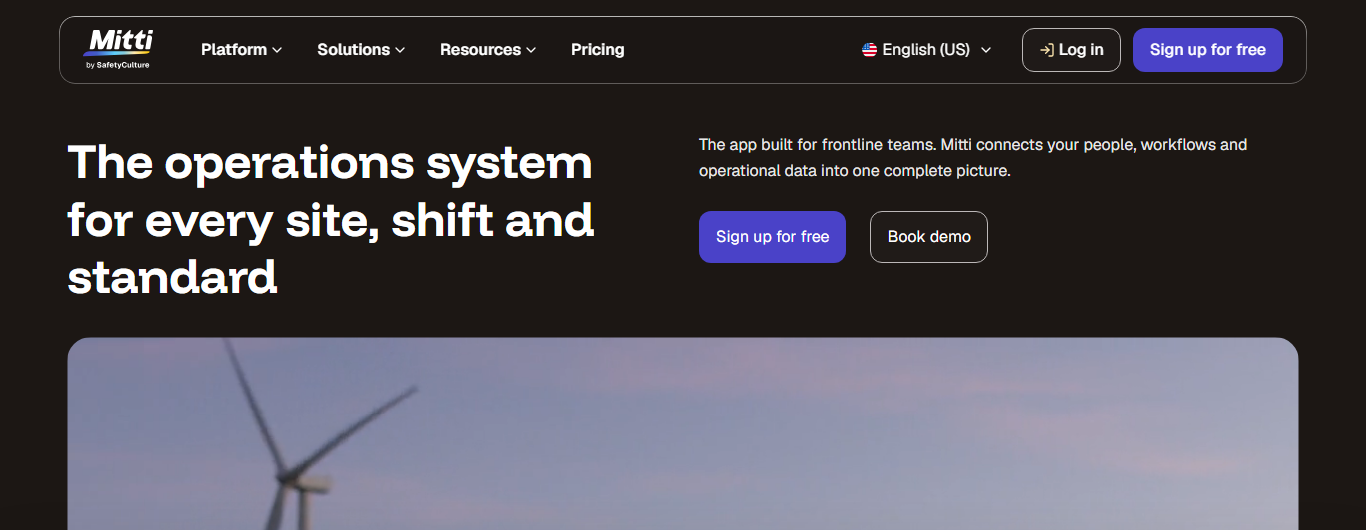
\includegraphics[width=0.85\linewidth]{Figures/cmp_safetyculture.png}
\caption{SafetyCulture (Mitti) платформын нүүр хуудас}
\label{fig:cmpsc}
\end{figure}

\subsection{Weekdone}
Weekdone нь OKR зорилго болон долоо хоногийн төлөвлөгөө, үр дүн, саадыг бичүүлж, багийн тайланг нэгтгэдэг. Долоо хоногийн тайлангийн дадлыг сайн хэрэгжүүлсэн боловч 5S, аудитын хэрэгсэлгүй~\cite{weekdone}.
\begin{figure}[H]
\centering
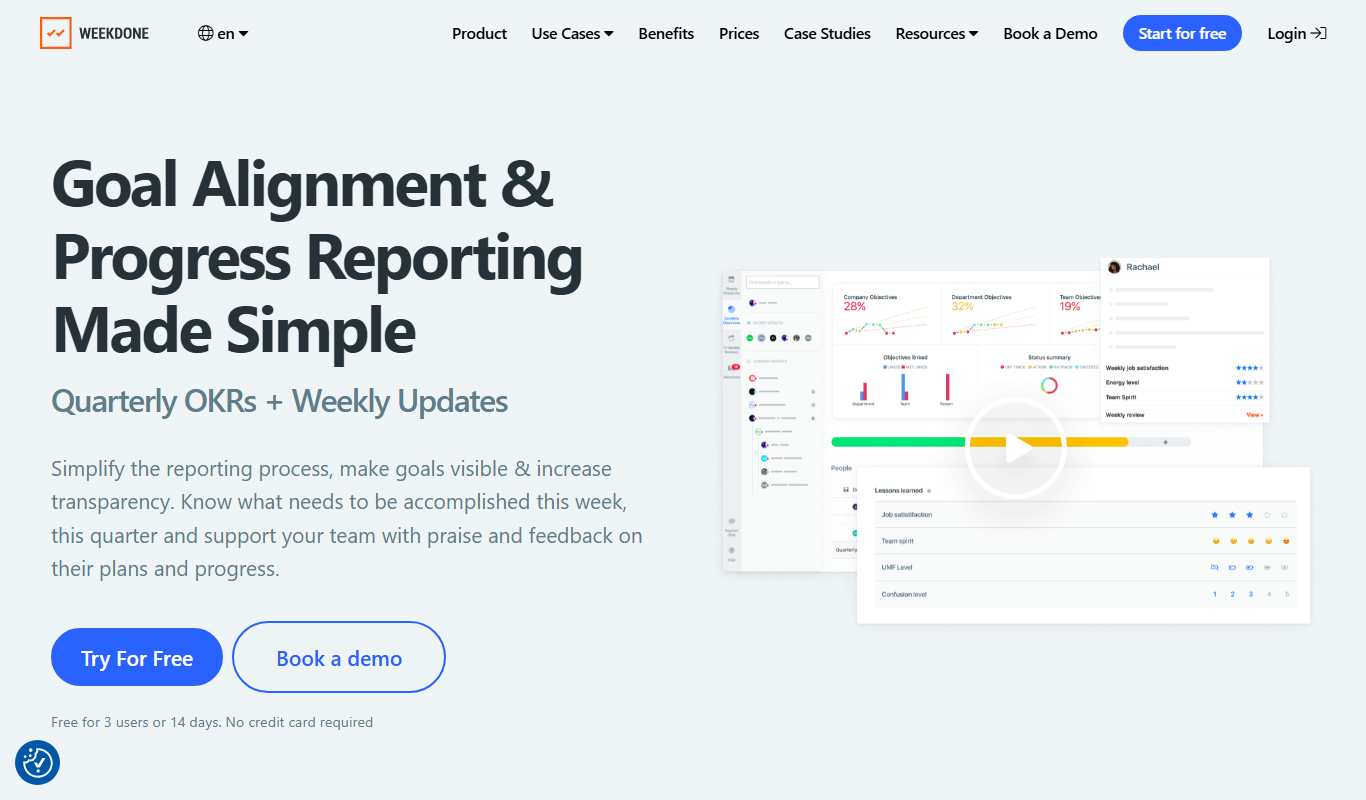
\includegraphics[width=0.85\linewidth]{Figures/cmp_weekdone.png}
\caption{Weekdone платформын нүүр хуудас}
\label{fig:cmpwd}
\end{figure}

\subsection{Asana}
Asana, Trello зэрэг ажлын удирдлагын системүүд ажил оноох, самбараар хянах, хугацаа сануулах боломжтой ч lean хэрэгсэл, аудит, талбайн удирдлага агуулдаггүй~\cite{asana}.
\begin{figure}[H]
\centering
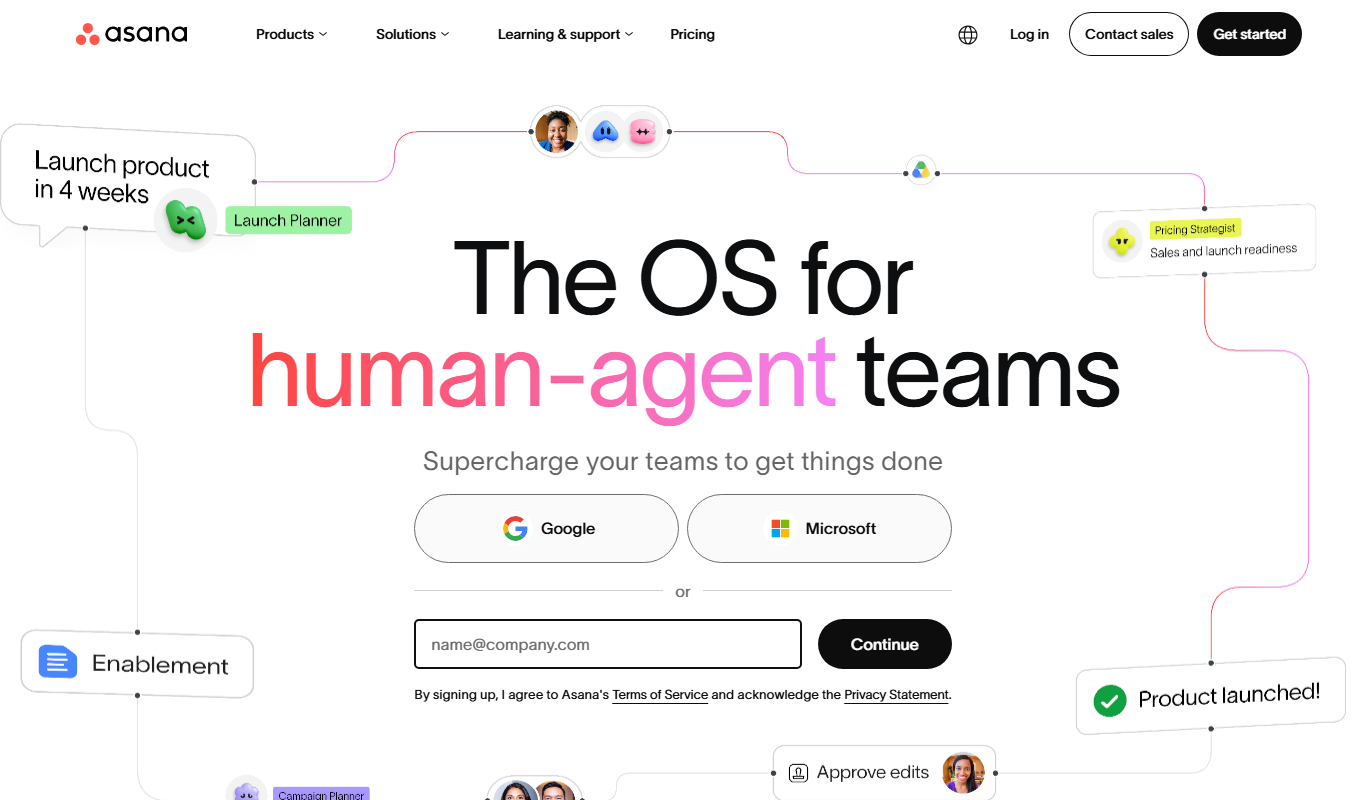
\includegraphics[width=0.85\linewidth]{Figures/cmp_asana.png}
\caption{Asana платформын нүүр хуудас}
\label{fig:cmpas}
\end{figure}

\subsection{KaiNexus}
KaiNexus нь тасралтгүй сайжруулалтын санаа, төслийг бүртгэж, үр нөлөөг хэмждэг платформ юм. Сайжруулалтын санааны урсгал сайн боловч аудит, сүлжээгүй горимгүй~\cite{kainexus}.
\begin{figure}[H]
\centering
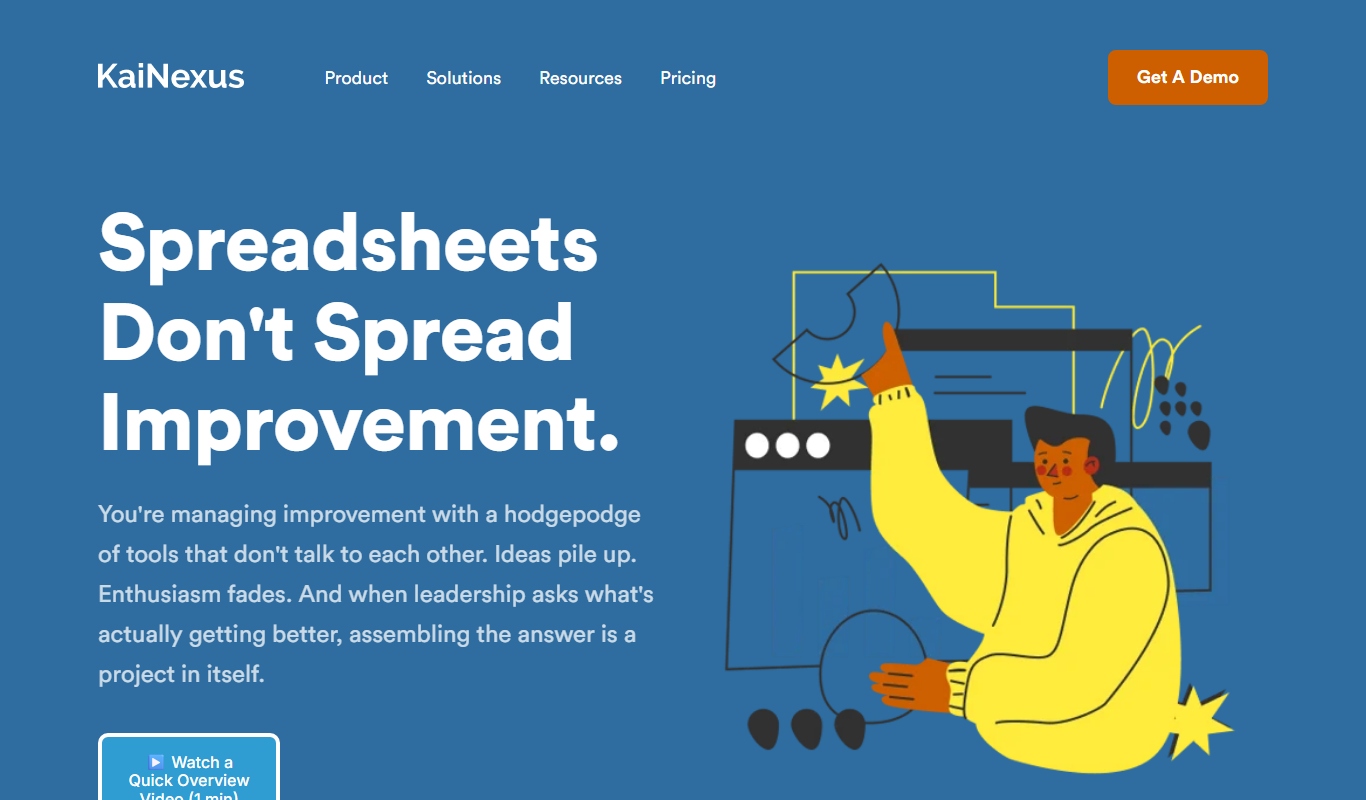
\includegraphics[width=0.85\linewidth]{Figures/cmp_kainexus.png}
\caption{KaiNexus платформын нүүр хуудас}
\label{fig:cmpkn}
\end{figure}

\subsection{Tervene}
Tervene нь шатлалт хурал, Gemba явалт, удирдагчийн стандарт ажил, харааны удирдлагын самбарыг цахимжуулсан үйлдвэрийн удирдлагын систем юм. Lean удирдлагын дадлыг хамгийн бүрэн хамардаг ч монгол хэлгүй, байгууллагын өөрийн серверт байршуулах боломжгүй~\cite{tervene}.
\begin{figure}[H]
\centering
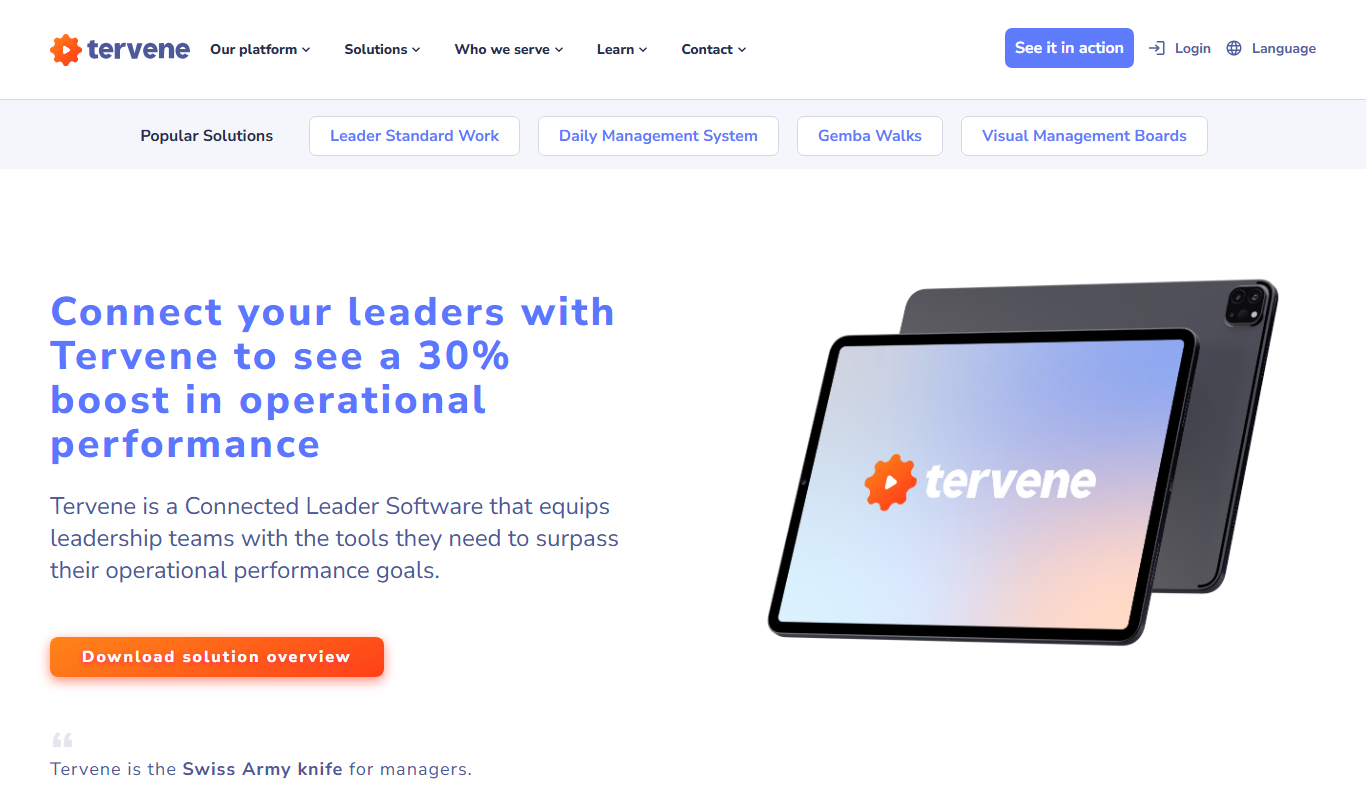
\includegraphics[width=0.85\linewidth]{Figures/cmp_tervene.png}
\caption{Tervene платформын нүүр хуудас}
\label{fig:cmptv}
\end{figure}

\subsection{Харьцуулалт ба SWOT шинжилгээ}


\begin{table}[H]
\centering
\caption{Ижил төстэй системийн боломжийн харьцуулалт}
\label{table:compare}
\begin{tabular}{|p{4.6cm}|c|c|c|c|c|c|}
\hline
\textbf{Боломж} & \rotatebox{90}{\textbf{SafetyCulture}} & \rotatebox{90}{\textbf{Weekdone}} & \rotatebox{90}{\textbf{Asana/Trello}} & \rotatebox{90}{\textbf{KaiNexus}} & \rotatebox{90}{\textbf{Tervene}} & \rotatebox{90}{\textbf{Энэ систем}} \\ \hline
Аудит, шалгах хуудас (утаснаас) & \yes & -- & -- & $\sim$ & \yes & \yes \\ \hline
Ажил оноох, хянах & $\sim$ & $\sim$ & \yes & \yes & \yes & \yes \\ \hline
Аудитаас автомат засах ажил & \yes & -- & -- & -- & $\sim$ & \yes \\ \hline
Сайжруулалтын санаа & -- & -- & -- & \yes & \yes & \yes \\ \hline
Өдөр тутмын хурлын самбар & -- & -- & -- & $\sim$ & \yes & \yes \\ \hline
Долоо хоногийн тайлан & -- & \yes & -- & -- & -- & \yes \\ \hline
Gemba явалтын бүртгэл & $\sim$ & -- & -- & -- & \yes & \yes \\ \hline
Сарын тайлан автоматаар & $\sim$ & $\sim$ & -- & $\sim$ & $\sim$ & \yes \\ \hline
Сүлжээгүй горим & \yes & -- & $\sim$ & -- & -- & \yes \\ \hline
Монгол хэл, өөрийн серверт & -- & -- & -- & -- & -- & \yes \\ \hline
\end{tabular}

\smallskip
{\small \yes -- бүрэн, $\sim$ -- хэсэгчлэн, -- -- байхгүй}
\end{table}

Хүснэгт~\ref{table:compare}-аас харахад SafetyCulture нь аудит, сүлжээгүй горимоороо, Weekdone нь долоо хоногийн тайлангаараа, KaiNexus, Tervene нь сайжруулалт болон lean удирдлагын дадлаараа давуу боловч эдгээрийг нэг дор, монгол хэл дээр, байгууллагын өөрийн серверт байршуулах боломжтой шийдэл байхгүй. Мөн эдгээр нь хэрэглэгч тус бүрээр гадаад валютаар төлбөртэй тул дотоодын байгууллагад зардал өндөр. Эдгээр системийн шилдэг туршлагыг (офлайн аудит, хариуцагчтай засах ажил, хурлын самбар, долоо хоногийн сануулга) энэхүү системд нэгтгэн тусгав.


Судалгааны үр дүнд үндэслэн хөгжүүлэх системийн давуу, сул тал, боломж, аюулыг Хүснэгт~\ref{table:swot}-д нэгтгэв.

\begin{table}[H]
\centering
\caption{Хөгжүүлэх системийн SWOT шинжилгээ}
\label{table:swot}
\begin{tabular}{|p{7cm}|p{7cm}|}
\hline
\textbf{Давуу тал (S)} & \textbf{Сул тал (W)} \\ \hline
\begin{itemize}[leftmargin=*,nosep]
\item Аудит, ажил, lean дадал нэг системд
\item Аудитаас засах ажил автоматаар үүснэ
\item Сүлжээгүй горим, монгол хэл
\item Өөрийн серверт байршуулах боломж
\end{itemize}
&
\begin{itemize}[leftmargin=*,nosep]
\item Хэрэглэгчийн бодит туршлага бага
\item Push мэдэгдэл хараахан байхгүй
\item Нэг хөгжүүлэгчтэй, дэмжлэгийн нөөц хязгаарлагдмал
\end{itemize}
\\ \hline
\textbf{Боломж (O)} & \textbf{Аюул (T)} \\ \hline
\begin{itemize}[leftmargin=*,nosep]
\item 5S, lean нэвтрүүлж буй байгууллага олон
\item Тайлан бэлтгэх цаг хэмнэх хэрэгцээ өндөр
\item AI ашиглан тайлан ноороглох
\end{itemize}
&
\begin{itemize}[leftmargin=*,nosep]
\item Гадаадын том системүүдтэй өрсөлдөх
\item Байгууллагын цахим шилжилтэд эсэргүүцэл
\item Хувийн мэдээллийн аюулгүй байдлын эрсдэл
\end{itemize}
\\ \hline
\end{tabular}
\end{table}

%-------------------------------------------------------------------------------
\section{Хэрэглэгчийн судалгаа}
% TODO: 5S, lean хэрэглэдэг байгууллагуудын ажилтнуудаас Google Form-оор судалгаа авч, үр дүнгийн графикуудыг
% Figures/survey*.png болгон энд оруулна. Үр дүнг зохиож бичихгүй.
Системийн шаардлагыг баталгаажуулах зорилгоор 5S, lean аргачлал хэрэглэдэг байгууллагуудын ажилтнуудаас онлайн асуулга авна. Асуулгын гол асуултууд:
\begin{enumerate}
    \item Та ажлын даалгаврыг голчлон ямар хэлбэрээр авдаг вэ? (ам, чат, имэйл, цаас, систем)
    \item 5S аудитын шалгах хуудсыг ямар хэлбэрээр бөглөдөг вэ?
    \item Аудитаар илэрсэн дутагдал засагдсан эсэхийг хэрхэн хянадаг вэ?
    \item Сарын тайлан бэлтгэхэд дунджаар хэдэн цаг зарцуулдаг вэ?
    \item Ажлын байранд интернэт тасалддаг уу?
    \item Сайжруулалтын санаагаа хаана, хэрхэн илэрхийлдэг вэ? Хариу авдаг уу?
    \item Ажлын системийг гар утаснаас ашиглах хэрэгцээ хэр байна вэ?
\end{enumerate}
Асуулгыг 2026 оны 10-р сард Google Forms-оор авч, хариултыг асуулт бүрээр график болгон нэгтгэнэ. Үр дүнг хоёрдугаар үзлэгт энэ хэсэгт тусгаж, шаардлагын жагсаалт болон тэдгээрийн эрэмбийг (Хүснэгт~\ref{table:fr}) шаардлагатай бол шинэчилнэ. Мөн туршилтын ажиллагааны төгсгөлд хэрэглэгчдээс SUS асуулга~\cite{brooke} авч, системийн хэрэглэхэд хялбар байдлыг 100 онооны хэмжүүрээр үнэлнэ.

%-------------------------------------------------------------------------------
\section{Системд тохирсон программ хангамжийн аргачлал}
Хөгжүүлэлтэд давталттай, өсөн нэмэгдэх (iterative and incremental) аргачлалыг сонгов~\cite{sommerville}. Захиалагчийн шаардлага эхнээсээ бүрэн тодорхой бус, туршилтын явцад өөрчлөгдөх магадлалтай тул давталт бүр нэг хэрэгцээг бүрэн (өгөгдлийн сан, API, вэб, гар утас, тест) хэрэгжүүлж, ажиллах хувилбар гаргана. Давталт бүр дараах алхмаас бүрдэнэ:
\begin{enumerate}[nosep]
    \item шаардлагыг тодорхойлох,
    \item зохиомжлох (өгөгдлийн загвар, API),
    \item хэрэгжүүлэх,
    \item автомат тест бичиж шалгах,
    \item захиалагчтай хянаж, дараагийн давталтыг төлөвлөх.
\end{enumerate}
Код бүрийг автомат тестээр хамгаалж, өөрчлөлт хийх бүрт бүх тестийг ажиллуулснаар өмнөх боломжуудыг эвдэхээс сэргийлнэ~\cite{beck}. Чанарын үзүүлэлтийг ISO/IEC 25010 стандартын функциональ тохирол, найдвартай байдал, хэрэглэхэд хялбар байдал, аюулгүй байдал, засварлагдах чанар гэсэн шинжүүдээр тодорхойлов~\cite{iso25010}.

%-------------------------------------------------------------------------------
\section{Технологийн тухай}
Технологийг хөгжүүлэлтийн хурд, нэг хэл дээр ажиллах боломж, урт хугацааны дэмжлэг, туршлага гэсэн шалгуураар сонгов.

\subsection{Front-End хөгжүүлэлтэд ашиглах технологиуд}
\begin{itemize}
    \item \textbf{React 18} -- компонентод суурилсан хэрэглэгчийн интерфейсийн сан~\cite{react}. Экосистем том, TypeScript-тэй сайн нийцдэг.
    \item \textbf{Vite} -- хурдан хөгжүүлэлтийн сервер ба бүтээх хэрэгсэл.
    \item \textbf{Tailwind CSS} -- utility класст суурилсан загварчлал; бараан горим, гар утасны дэлгэцэд тохируулахад хялбар.
    \item \textbf{i18next} -- монгол, англи хэлний орчуулга.
\end{itemize}

\subsection{Back-End хөгжүүлэлтэд ашиглах технологиуд}
\begin{itemize}
    \item \textbf{NestJS 11} -- TypeScript дээрх модульчлагдсан сервер талын фреймворк~\cite{nestjs}. Dependency injection, guard-аар эрх шалгах, cron үйлдлийг дэмждэг.
    \item \textbf{PostgreSQL} -- харилцааны өгөгдлийн сан~\cite{postgres}. Гадаад түлхүүрээр бүрэн бүтэн байдлыг хангаж, JSONB төрлөөр уян хатан өгөгдөл (5S бүс, шалгах хуудас) хадгална.
    \item \textbf{TypeORM} -- объект-харилцааны буулгалт (ORM); схемийн өөрчлөлтийг migration файлаар хувилбарчилна.
    \item \textbf{JWT} -- төлөвгүй нэвтрэлт; вэб, гар утас хоёрт ижил ажиллана~\cite{jwt}.
    \item \textbf{Docker Compose} -- nginx, API, PostgreSQL-ийг нэг тохиргоогоор байршуулна.
\end{itemize}

\subsection{Гар утасны хөгжүүлэлтэд ашиглах технологиуд}
\begin{itemize}
    \item \textbf{Flutter (Dart)} -- нэг кодоор Android, iOS аппыг бүтээх хүрээ~\cite{flutter}.
    \item \textbf{Provider} -- төлөв удирдлага; \textbf{Dio} -- HTTP клиент.
    \item \textbf{SharedPreferences} -- сүлжээгүй үед бүртгэлийн дарааллыг (outbox) хадгална.
\end{itemize}

\begin{table}[H]
\centering
\caption{Технологийн сонголт ба харьцуулсан хувилбарууд}
\label{table:tech}
\begin{tabular}{|p{2.4cm}|p{3.2cm}|p{2.8cm}|p{5.2cm}|}
\hline
\textbf{Давхарга} & \textbf{Сонгосон} & \textbf{Хувилбар} & \textbf{Үндэслэл} \\ \hline
Backend & NestJS 11 & Express, Django & Модульчлагдсан бүтэц, guard, вэбтэй нэг хэл \\ \hline
Өгөгдлийн сан & PostgreSQL & MySQL, MongoDB & Бүрэн бүтэн байдал, JSONB, migration \\ \hline
Вэб & React 18 & Angular, Vue & Компонент, экосистем, хурд \\ \hline
Гар утас & Flutter & React Native & Нэг код, тогтвортой гүйцэтгэл, widget тест \\ \hline
Байршуулалт & Docker Compose & Шууд суулгах & Орчин ижил, өөрийн серверт хялбар \\ \hline
\end{tabular}
\end{table}

\section*{Бүлгийн дүгнэлт}
Энэ бүлэгт бүтээмжийн аргачлалуудын онолыг судалж, тэдгээрийг дадал болгоход сануулга, хяналтын механизм шаардлагатайг тодорхойлов. Ижил төстэй таван системийг харьцуулж, SWOT шинжилгээ хийж, аудит, ажлын удирдлага, lean дадлыг нэг дор, монгол хэл дээр нэгтгэсэн шийдэл байхгүйг тогтоов. Мөн давталттай хөгжүүлэлтийн аргачлал, NestJS, PostgreSQL, React, Flutter технологийг сонгосон үндэслэлээ тайлбарлав.
